\documentclass[a4paper,12pt]{scrartcl}
% \setcounter{secnumdepth}{3}
% \setcounter{tocdepth}{5}

% \makeatletter
% \renewcommand\section{\newpage\@startsection {section}{1}{\z@}%
%                                    {-3.5ex \@plus -1ex \@minus -.2ex}%
%                                    {2.3ex \@plus.2ex}%
%                                    {\normalfont\Large\bfseries}} 
% \renewcommand\paragraph{\@startsection{paragraph}{4}{\z@}%
%                                      {-3.25ex\@plus -1ex \@minus -.2ex}%
%                                      {0.0001pt \@plus .2ex}%
%                                      {\normalfont\normalsize\bfseries}}
% \renewcommand\subparagraph{\@startsection{subparagraph}{5}{\z@}%
%                                      {-3.25ex\@plus -1ex \@minus -.2ex}%
%                                      {0.0001pt \@plus .2ex}%
%                                      {\normalfont\normalsize\bfseries}}
% \makeatother

\newcommand\doctype{Technische Dokumentation}
\newcommand\supervisor{Prof. Dr. phil. Hugo M. Kehr}
\newcommand\advisor{Dipl. Psych. Stefan Engeser}
\newcommand\deliverydate{4. M{\"a}rz 2011}

\newcommand*{\code}[1]{\texttt{#1}}% style for code insertions

\usepackage[T1]{fontenc}
\usepackage{lmodern}


% \usepackage{pstricks}
% \usepackage{pst-plot}
% \usepackage{auto-pst-pdf}

\usepackage{bibgerm}
\usepackage[hang,flushmargin]{footmisc}
\usepackage[printonlyused]{acronym}
\usepackage{url}
\usepackage[utf8]{inputenc}
\usepackage{graphicx}
\usepackage[hang,small,bf]{caption}
\usepackage{styles/tumlogo}
\usepackage{setspace}
\usepackage[german,english]{babel}
\usepackage{needspace}
\usepackage{fancyhdr}
\pagestyle{fancy}
\headheight 35pt
\lhead{\nouppercase{\leftmark}}
\rhead{
\includegraphics[width=0.5cm]{styles/info.pdf}}


% \selectlanguage{english}

% \usepackage{hyperref} % sorgt für für Hyperlinks in PDF-Dokumenten
\usepackage[plainpages=false,pdfpagelabels, bookmarks=true]{hyperref}                                             %. hyper-references for ps2pdf 
% \usepackage[ocgcolorlinks]{hyperref}     % sorgt für farbige für Hyperlinks, die beim Ausdruck schwarz sind
\hypersetup{
    breaklinks=true
    unicode=false,          % non-Latin characters in Acrobat’s bookmarks
    pdftoolbar=true,        % show Acrobat’s toolbar?
    pdfmenubar=true,        % show Acrobat’s menu?
    pdffitwindow=true,      % page fit to window when opened
    pdftitle={},    % title
    pdfauthor={},     % author
    pdfsubject={},   % subject of the document
    pdfnewwindow=true,      % links in new window
    pdfkeywords={}, % list of keywords
    pdfstartview={FitH},
    colorlinks=true,       % false: boxed links; true: colored links
%     linkcolor=red,          % color of internal links
%     citecolor=green,        % color of links to bibliography
%     filecolor=magenta,      % color of file links
%     urlcolor=cyan           % color of external links
    linkcolor=black,          % color of internal links
    citecolor=black,        % color of links to bibliography
    filecolor=black,      % color of file links
    urlcolor=black           % color of external links
}

\makeatletter
\g@addto@macro\UrlBreaks{\do\a\do\b\do\c\do\d\do\e\do\f\do\g\do\h\do\i%
\do\j\do\k\do\l\do\m\do\n\do\o\do\p\do\q\do\r\do\s\do\t\do\u\do\v\do\w%
\do\x\do\y\do\z\do\&\do\1\do\2\do\3\do\4\do\5\do\6\do\7\do\8\do\9\do\0}
%\def\do@url@hyp{\do\-}
\g@addto@macro\UrlSpecials{\do\/{\mbox{\UrlFont/}\hskip 0pt plus 1pt}}
\makeatother

\usepackage{cite}

\widowpenalty=10000
\clubpenalty=10000

\parindent 0pt % keine Absatzeinrückung
\parskip 6pt % aber danach ein gewisser Abstand

\graphicspath{{graphics/}}

% \sloppy

%
% der Befehl \hypenation versteht keine Sonderzeichen, also weder ä
% noch "a noch \"a. Wörter die derartige Zeichen enthalten müssen
% direkt im Text getrennt werden, z.B. Wör\-ter
%
\hyphenation{Luft-ma-tra-ze} % in dieses File kommen Wörter die Latex nicht richtig trennt

\begin{document}

\thispagestyle{empty}

\vspace{4cm}
\begin{center}
\oTUM{4cm}\\ 
\vspace{5mm}     
\huge FAKULT{\"A}T F{\"U}R INFORMATIK\\
und\\
FAKULT{\"A}T F{\"U}R WIRTSCHAFTSWISSENSCHAFTEN\\

 
\vspace{0.5cm}
\large DER TECHNISCHEN UNIVERSIT{\"A}T M{\"U}NCHEN\\
\vspace{1mm}
\end{center}

\vspace{10mm}

\begin{center}
\Large \doctype
\vspace{15mm}

\begin{spacing}{1.5}
\huge\bf Flowgame\\%[3ex]
\end{spacing}

\vspace{10mm}
\LARGE Philipp Reichart, Barbara K{\"o}hler,\\ Christopher
H{\"u}bner und Sebastian V{\"o}st

\vspace{10mm}

\begin{figure}[h!]
\centering

\includegraphics[height=3cm]{styles/info.pdf}
\end{figure}

\end{center}

\thispagestyle{empty}

\vspace{8mm}
\begin{center}
\oTUM{4cm}

\vspace{5mm}     
\huge FAKULT{\"A}T F{\"U}R INFORMATIK\\ 
und\\
FAKULT{\"A}T F{\"U}R WIRTSCHAFTSWISSENSCHAFTEN\\ 
\vspace{0.5cm}
\large DER TECHNISCHEN UNIVERSIT{\"A}T M{\"U}NCHEN\\
\end{center}

\vspace{3mm}

\begin{center}
\Large \doctype
\vspace{2mm}

\begin{spacing}{1.3}
\Huge Flowgame
\vspace{3mm}
\end{spacing}

\begin{tabular}{ll}
\Large Autoren:     & \Large Philipp Reichart, Barbara K{\"o}hler,\\ 
\Large 			  & \Large Christopher H{\"u}bner und Sebastian V{\"o}st\\[2mm]
\Large Aufgabensteller: & \Large \supervisor \\[2mm]				
\Large Betreuer:	   & \Large \advisor    \\[2mm]
\Large Datum:       & \Large \deliverydate
\end{tabular}


\vspace{3mm}

\begin{figure}[hb!]
\centering

\includegraphics[height=3cm]{styles/info.pdf}
\end{figure}


\end{center}

% \include{disclaimer}
% 
% \pagenumbering{roman}
% \thispagestyle{plain}
% 
% 
% \selectlanguage{english}
% \thispagestyle{plain}
% \begin{abstract}
% \noindent english abstract
% \end{abstract}
% \clearpage

\selectlanguage{german}
% \begin{abstract}
% \noindent Deutsche Kurzfassung
% \end{abstract}
% \clearpage


\tableofcontents
\clearpage

\pagenumbering{arabic}


\clearpage


\section{Funktionale Anforderungen}
Der Zustand des "`Flow"' ist ein psychologisches Phänomen, das bei diversen verschiedenen
Tätigkeiten zu beobachten ist. Computerspiele zählen zu diesen Tätigkeiten, da sie die
grundlegenden Anforderungen zur Generierung von Flow erfüllen: Der Spieler muss aktiv
sein und einer gewissen Herausforderung gegenüberstehen.\newline
In diesem Projekt soll also zunächst einmal ein Spiel entwickelt werden, das den Spieler
potentiell in einen Zustand des Flow bringt, oder, so gewollt, in einen Zustand des "`Nicht-
Flow"'.

Als Spielkonzept wurde ein simples Setting gewählt: Der Spieler steuert ein Raumschiff
und muss dabei Hindernissen ausweichen und Boni aufsammeln, die mit variabler
Geschwindigkeit auf ihn zukommen. Anhand der Geschwindigkeit lässt sich hierbei der
Schwierigkeitsgrad regulieren, um so gezielt Unterforderung, Überforderung oder ideale
Anforderungen schaffen zu können.

Zur Navigation im Spiel ist es nötig, zunächst ein Hauptmenü zu integrieren, in dem man
wählen kann, ob man eine Runde beginnen, die Highscores einsehen, die
persönlichen Einstellungen ändern oder die Credits ansehen möchte.\newline
Bei neuen Spielern wird zunächst ein Persönlichkeitsprofil angelegt, in dem der Spieler
mithilfe eines Fragebogens gewisse persönliche Charakteristika angibt, die zur Auswertung
der erhobenen Daten hilfreich sind.\newline
Ist dies geschehen, kann ein Spiel beginnen. Dieses ist aufgeteilt in mehrere Runden, in
denen zunächst die "`Tagesform"', also die Leistungsfähigkeit für diese Runde gemessen
wird. Dies ermöglicht, trotz Lerneffekten oder anderen Einflüssen, wie etwa Müdigkeit oder
mangelnde Konzentration, in jeder Situation die idealen Anforderungen zu
generieren.\newline
Daraufhin folgen drei Runden, in denen sich verschiedene
Anforderungsstufen abwechseln. Um die Rahmenbedingungen für alle Spieler gleich zu halten, hat jede Runde eine fixe
Dauer.

%\usepackage{graphics} is needed for \includegraphics
\begin{figure}[htp]
\begin{center}
  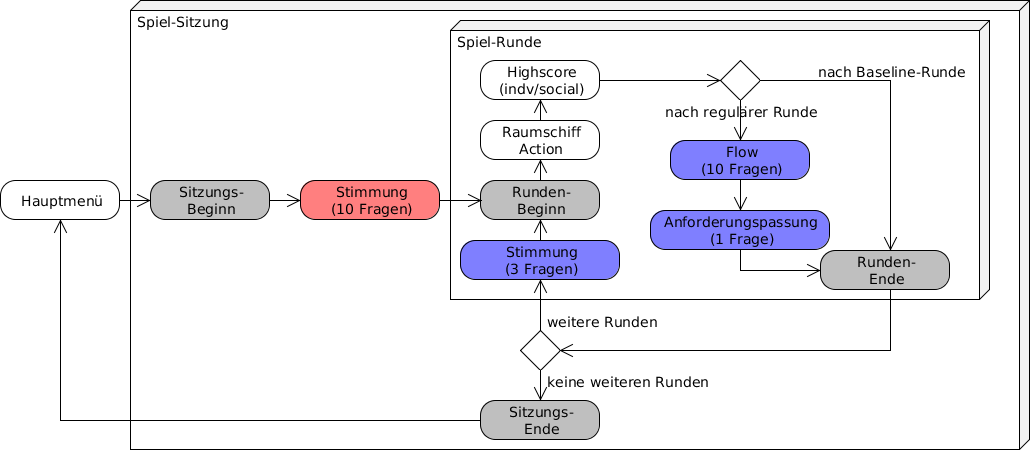
\includegraphics[width=\textwidth]{SpielablaufClient.png}
  \caption{Clientseitiger Spielablauf}
  \label{fig:ClientSpielablauf}
\end{center}
\end{figure} 

Das ganze Spiel ist, um etwas Atmosphäre zu erzeugen, in eine Rahmengeschichte
eingebettet, die den Spieler in ein Science-Fiction-Szenario hineinversetzt und ihm vor jeder
Runde eine Aufgabe gibt, die er zu erfüllen hat und ihm am Ende der Runde über seine
Erfolge berichtet.\newline
Zusätzlich wird das Befinden in einer Art "`Rennen"' durch ein schnelles, futuristisch
erscheinendes Musikstück unterstützt, das während den Runden abgespielt wird und
speziell hierfür komponiert wurde.

Um anhand hiervon nun festzustellen, ob ein Spieler Flow erfährt, muss eine Methode
gewählt werden, um dies zu messen.\newline
Das Mittel der Wahl sind hier Teile der Fragebögen der von Engeser entwickelten
FKS\footnote{TODO: Erklärung}, die zwischen den Spielrunden eingeblendet
werden, sowie weitere Fragen zur Anforderungspassung, um das subjektive Empfinden der angepassten Schwierigkeit
überprüfen zu können. Die Beantwortung dieser Fragen erfolgt durch einen stufenlos
anpassbaren Schieberegler, der zwischen zwei gegensätzlichen Adjektiven nach
Belieben eingestellt werden kann. Ein Lerneffekt beim Beantworten der Fragen oder eine
Automatisierung ebendessen wird verhindert, indem die Fragen in randomisierter
Reihenfolge erscheinen. Außerdem
wird die Dauer der Beantwortung eines jeden Fragebogens gemessen, was Rückschlüsse
darauf zulässt, ob der Spieler nur zufällig etwas angeklickt, oder die Fragen tatsächlich
gelesen und gewissenhaft beantwortet hat.

Als Plattform für das Spiel wurde das soziale Netzwerk Facebook gewählt, das die
Integration von vielfältigen Anwendungen erlaubt. Mit Facebook lassen sich vielerlei Daten,
die der Spieler auf seinem Profil ohnehin angegeben hat, wie etwa Alter, Geschlecht und
Herkunft, nutzen. Diese Daten können dann automatisiert und ohne zusätzliche Angaben
erfasst werden und in die Auswertung einfließen.\newline
Außerdem ist es hier möglich,die Leistungen verschiedener Teilnehmer zu vergleichen
und in einer Highscore darzustellen. Das erlaubt die Untersuchung von Unterschieden der
Leistung von individuell und sozial motivierten Spielern.

Zuletzt wurde eine einfache und umfassende Möglichkeit der erhobenen Daten gefordert.
Dies ließ sich durch eine direkte Einspeisung in eine SQL-Datenbank realisieren. Dies hat
den Vorteil, dass die Daten elektronisch und delokalisiert vorliegen und ein Zugriff über das
Internet möglich ist. Hierfür steht ein browserbasierter Client zur Verfügung. Zudem lässt
sich die Datenbank im SPSS-Format exportieren.


\section{Nicht-Funktionale Anforderungen}
Um gleiche Rahmenbedingungen und damit eine Vergleichbarkeit zwischen verschiedenen
Spielern und Spielen nicht von vornherein zu verhindern, muss der Spielablauf in
eine möglichst kontrollierte Umgebung eingebettet werden. Das bedeutet, dass sich
verschiedene Spiele nicht zu stark voneinander unterscheiden dürfen. Ein kritischer Punkt
hierfür ist die Dauer einer Runde. Es steht zu befürchten, dass Spieler trotz gleichem
Schwierigkeitsgrad signifikant unterschiedliche Erlebnisse berichten, wenn sich die
Spieldauer in großem Maße unterscheidet. Daher wurde für jede Runde eine fixe Spieldauer
von 120 Sekunden festgelegt. Diese Dauer lässt sich auch nicht durch ein "`verlieren"'
oder "`sterben"', wie ich anderen Spielen üblich verkürzen. Man muss in diesem Spiel zwar
Hindernissen ausweichen, diese führen aber nie zum Spieltod, sondern immer nur zu einer
Verringerung der Endpunktzahl. Diese Endpunktzahl übt als Maß zur Leistungsmessung für
den Spieler einen Anreiz für hohe Performance und damit Anstrengung aus. Daher ist es
sinnig, dass der Spieler neben dem zwanghaften Ausweichen von Hindernissen auch noch
eine Anforderung darin hat, gleichzeitig möglichst viele Bonuspunkte zu sammeln.

Obwohl es sich hierbei um ein psychologisches Experiment handelt, ist es wünschenswert,
dass der Spieler nicht das Gefühl hat, in einem Labor an einer Datenerhebung
teilzunehmen, sondern vielmehr ein Spiel spielt, um sich die Zeit zu vertreiben oder
ähnliches. Daraus resultieren die oben genannten Anforderungen, das Spiel mit
Rahmengeschichte und Musik auszustatten, da dies von einem Spiel erwartet wird und
ein Fehlen solcher Details zu einem verfälschten Empfinden führen könnte. Ebenso
gehört dazu, dass die Fragebögen möglichst gut ins Spiel eingebettet werden und ihre
Beantwortung durch eine Rahmengeschichte eingepasst wird. Müssten die Fragebögen
extern bearbeitet werden, etwa per Papier oder durch einen weiteren Webclient, so wäre es
unvermeidlich, dass der Spieler sich mehr als Proband empfindet.

Ziel des Projekts ist außerdem, möglichst viele Datensätze zu erheben, also möglichst viele
Menschen zu erreichen. Dafür muss das Spiel allerdings einige Anforderungen erfüllen
und nicht zu hohe Hürden an den Benutzer stellen. Das bedeutet zunächst eine möglichst
einfache Bedienbarkeit. Angestrebt waren lediglich vier Tasten, nämlich die Pfeiltasten, die
ausreichend sind, das Raumschiff nach oben, unten, links und rechts zu steuern. Ebenso
dazu gehört es, das Spiel möglichst kurzweilig zu gestalten. Ein Spiel (bestehend ja aus
vier Runden) sollte weniger als 15 Minuten dauern, um der kurzlebigen Internetkultur zu
entsprechen. Im Internet wird oft kurz "`zwischendurch"' oder beim Warten gespielt und eine
längere Dauer würde das Spiel hierfür komplett ausschließen. Außerdem ist es wichtig, den
Anforderungen der verschiedenen Betriebssysteme, die verbreitetsten sind Windows, Mac/OSX und Linux, gerecht zu werden. Teile der potentiellen Teilnehmerschaft wegen ihres
Betriebssystems ausschließen zu müssen, wäre äußerst unerfreulich. Ebenso gibt es keinen
Grund, das Projekt auf den deutschen Raum zu beschränken. Eine Sprachunterstützung
von Englisch und Deutsch soll die Anzahl der potentiellen Teilnehmer noch einmal
signifikant erhöhen. Dazu wurden die Standards der in der Informatik so genannten "`I18N"'
(kurz für Internationalisierung) eingehalten. Teil dessen ist, dass Programmteile, die sich
bei unterschiedlichen Sprachversionen unterscheiden, nicht im Quellcode stehen, sondern
einfach durch den Austausch von bestimmten Dateien ersetzt werden können. Dies
ermöglicht die Erweiterung auf andere Sprachräume, ohne das eigentliche Programm zu
ändern.

\section{Architektur}
\subsection{Client-Server}
Die grundlegende Architektur des Spiels ist Client-Server-basiert, wobei ein auf
Facebook angezeigtes Applet den Client und ein auf einem eigenen Server laufender
Webcontainer den Server darstellen. Die Kommunikation zwischen Client und Server erfolgt
ausschließlich über HTTP\footnote{Hypertext Transfer Protocol -- Protokoll zur
Übertragung von Daten über ein Netzwerk, hauptsächlich für die Übermittlung
von Webseiten eingesetzt.}. Programmcode für Funktionalitäten, die spezifisch
für Client (Benutzerschnittstelle, 3D-Umgebung, Facebook-Anbindung) und Server (Datenbank- Anbindung, Programmlogik) sind, ist voneinander unabhängig, lediglich der Programmcode für das gemeinsam genutzte Datenmodell ist beiden Seiten bekannt. Dies entspricht der üblichen Praxis, reduziert unerwünschte Seiteneffekte und ergibt eine klare Trennung der
Verantwortlichkeiten.

\subsection{Subsystemzerlegung}
TODO Christopher, Phil

\subsection{Datenmodell (Klassen / UML)}
TODO Christopher, Phil

\subsection{Datenbankmodell (Tabellen / ER)}
TODO Christopher, Phil

\section{Technologien}
Um den Entwicklungsaufwand für ein plattformübergreifendes Spiel möglichst gering
zu halten, haben wir uns entschieden, dass Spiel in Java umzusetzen, da es für alle
verbreiteten Betriebssysteme verfügbar ist und eine solide Bibliothek an Funktionen mit sich
bringt.

Serverseitig läuft eine Webanwendung auf Basis von Struts 2 und Servlets/JSPs, die
über EclipseLink als JPA\footnote{Java Persistence API, eine Schnittstelle um
Java-Objekte-Graphen in gebräuchliche relationale Datenbanksysteme
abzubilden.}-Provider mit einer Datenbank kommuniziert, um Spieldaten zu speichern. Für die Kommunikation mit dem clientseitigen Spiel wird ein auf serialisierte Java-
Objekte aufbauender RPC-Mechanismus über HTTP angewandt.

Clientseitig läuft ein Applet, dass über Java3D die 3D-Umgebung und über Swing die
Benutzerschnittstelle anzeigt. Beide Bibliotheken abstrahieren die zugrundelegenden
Techniken stark, was eine komfortable Entwicklung komplexer 3D-Umgebungen und
Benutzerschnittstellen ermöglicht. Für die Anbindung an Facebook wird im Applet eine
weitere Bibliothek verwendet, die aufgrund von Sicherheitseinschränkungen (Same Origin
Policy) alle Aufrufe an das Facebook API über den Spielserver abwickelt.

\section{Implementierung}
\subsection{Baselinemessung und Adaptive Rundenzeiten}
Für die Erzeugung und Messung von Flow bzw. Unter- und Überforderung passt sich das
Spiel dem Spieler an. Dazu findet bei jedem Durchgang, einer sogenannten Session,
zunächst eine Messung der Baseline statt. Diese Baseline stellt die vermutete ideale
Anforderung an einen Spieler dar. Alle weiteren Runden werden im Verhältnis zur Baseline
im Schwierigkeitsgrad variiert.

In diesem Kapitel wird zunächst kurz die Messung der Baseline erläutert und
Schwierigkeiten die dabei auftreten können. Anschließend wird gezeigt, wie die
Geschwindigkeit der übrigen Runden aus der Baseline errechnet werden kann.
Baselinemessung

Bei der Baselinemessung soll erreicht werden, dass man die ideale Spielschwierigkeit für
einen Spieler ermittelt. Diese besteht prinzipiell aus den drei Komponenten Geschwindigkeit,
Verhältnis von Diamanten zu Asteroiden und Abstand zwischen den Asteroiden. Der
Einfachheit halber wird in unserem Experiment ausschließlich die Geschwindigkeit variiert,
eine Anpassungen der beiden anderen Parameter könnte aber analog erfolgen.

Die Passung soll ermittelt werden, indem zunächst alle auf der gleichen Geschwindigkeit
starten. Nach und nach wird die Geschwindigkeit erhöht, bis der Spieler nicht mehr mithalten
kann. An diesem Punkt wird wieder abgesenkt, bis es anscheinend deutlich zu einfach
wird. Dies wird in mehreren Iterationen über zwei Minuten hinweg wiederholt, wobei
der Ausschlag nach und nach kleiner wird und sich auf einer bestimmten Schwierigkeit
einpendelt. Die Baseline ist dann die Schwierigkeit oberhalb derer sich der
Spieler 50\% der Zeit halten konnte. Dieses Verhalten führt zu dem in Abbildung x dargestellten typischen
Verlauf.

%\usepackage{graphics} is needed for \includegraphics
\begin{figure}[htp]
\begin{center}
  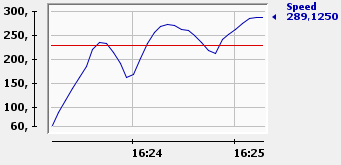
\includegraphics[width=0.6\textwidth]{Baseline.png}
  \caption[Baselinemessungsverlauf]{Baselinemessung Verlauf (blaue Linie),
  gemessene Baseline (rote Linie)}
  \label{fig:Baseline}
\end{center}
\end{figure} 

Als erstes muss also zunächst bestimmt werden, ob die Schwierigkeit zu einem gegebenen
Moment zu groß oder zu klein ist. Dazu speichert die Klasse Trend, zu wieviel Prozent
der Spieler mit einem bestimmten Objekt (Diamant oder Asteroid) kollidiert ist bzw. ihm
ausgewichen ist. Es wird jeweils ein lang-, mittel- und kurzfristiger Trend ermittelt, sodass
die Entscheidung nicht nur anhand der letzten Aktionen des Spelers getroffen werden.
Der langfristige Trend bezieht sich hierbei auf die letzten 30 passierenden Objekte.
Mittelfristig sind es die letzten 10 und für den kurzfristigen Trend werden nur die letzten 3
beachtet.
Beispiel: Es sind 10 Objekte in der folgenden Reihenfolge vorbeigeflogen, wobei ein (K)
bedeutet, dass der Spieler mit ihnen kollidiert ist:
\begin{enumerate}
\item Asteroid
\item Asteroid
\item Diamant (K)
\item Asteroid
\item Diamant (K)
\item Diamant
\item Diamant (K)
\item Asteroid (K)
\item Asteroid (K)
\item Diamant
\end{enumerate}
Dann ist der kurzfristige Trend, dass der Spieler mit 2 Asteroiden kollidiert
ist (Rate 100\%) und keinen Diamanten gesammelt hat (0\%), was eine Überforderung vermuten lässt.
Der mittelfristige Trend ist mit 2 Asteroiden (40\%) und 4 Diamanten (80%)
dagegen deutlich ausgewogener.

Aus dieser Information muss nun abgeschätzt werden, wann das Spiel langsamer und wann
es schneller werden sollte. Hierfür wurden mehrere verschiedene Methoden getestet. Im
Folgenden wird lediglich die beschrieben, die tatsächlich verwendet wurde, da sie sich als
am exaktesten herausgestellt hat.

Bis der Spieler mindestens zehn Objekte passiert hat wird die Geschwindigkeit einfach
immer gesteigert, da man bis zu diesem Moment noch nicht genug Daten hat, um
eine individualisierte Entscheidung zu treffen. Danach richtet sich die Anpassung der
Geschwindigkeit nach den gemessenen Trends. Kollidiert der Spieler mit einem Asteroiden
oder schafft er es nur 1/3 der Asteroiden aufzusammmeln so wird kurz abgebremst.
Sammelt er dagegen erfolgreich mehr als 2/3 der Diamanten, so wird sehr stark
beschleunigt. Sammelt er mittelfristig zumindest noch mehr als 1/3 der
passierenden Diamanten so wird leicht beschleunigt. Wenn keine dieser Bedingungen zutrifft, so bleibt alles gleich schnell. Dieses
Verhalten wird von der FunctionStrategy2 gesteuert.

Nun bleibt die Frage, wie stark beschleunigt oder gebremst werden soll. Am einfachsten
erscheint es unabhängig von der aktuellen Geschwindigkeit, diese um einen fixen Betrag
zu erhöhen oder zu reduzieren. Als dies mit Spielern getestet wurde haben wir jedoch
festgestelt, dass bei höherer Ausgangsgeschwindigkeit schon kleine Beschleunigungen
sich sehr drastisch anfühlen, während bei niedrigeren Geschwindigkeiten die
Geschwindigkeitserhöhung größer sein muss, um überhaupt wahrgenommen zu werden.

Um möglichst einfach mehrere verschiedene Modelle testen zu können wird deshalb der
Betrag der Erhöhung aus einer Funktion ermittelt. Die Funktion bildet eine Position auf
eine Geschwindigkeit ab. Zu Beginn einer Baselinerunde startet der Spieler an Position
0. Soll das Spiel schneller werden, so wird die Position erhöht, anders gesenkt. Die neue
Geschwindigkeit ergibt sich aus dem Wert der Funktion an der neuen Position.

Am besten hat sich die Funktion $\max(240 \tanh(\frac{x}{5000})+60,
30)$ erwiesen. Sie ist monoton steigend und bewegt sich zwischen dem niedrigsten
Wert (30) und nähert sich langsam an 300. Bei dieser Funktion sind die Anpassungen 
bei langsamen Geschwindigkeiten deutlicher sind als bei hohen Geschwindigkeiten.

%\usepackage{graphics} is needed for \includegraphics
\begin{figure}[htp]
\begin{center}
  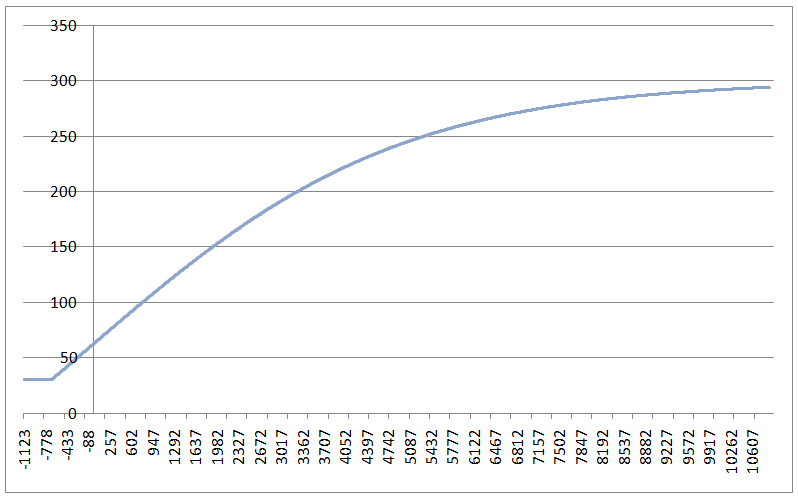
\includegraphics[width=0.8\textwidth]{BaselineFunktion.png}
  \caption[Grundlagenfunktion Baselinemessung]{Funktion die als Grundlage für
  die Baselinemessung verwendet wird.\\ TODO Vektorgrafik}
  \label{fig:BaselineFunktion}
\end{center}
\end{figure} 

Jede Änderung der Geschwindigkeit wird im SpeedChangeBehavior angestossen. Bei der
Baselinemessung merkt sich das Spiel jeden Wert und bestimmt zum Schluss die Baseline
aus dem Median dieser Werte.

Ausgehend von der Baseline werden die Geschwindigkeitenfür die folgenden drei Runden
folgendermaßen bestimmt:\\
Stufe 1 (Baseline - 60 + Baseline*0,7)/2\\
Stufe 2 (Baseline - 0 + Baseline*1)/2\\
Stufe 3 (Baseline + 60 + Baseline*1,13)/2\\

Im Quellcode wurden diese wiederum durch Funktionen dargestellt. Bei der
ConstantFunction bleibt die Geschwindigkeit über eine Runde hinweg konstant.
Die Anfangsgeschwindigkeit wird einmalig anhand der Baseline errechnet. Für die
kontinuierliche Bedingung wird eine passende LinearFunction benötigt. Hierbei muss
sich nicht nur der Schnittpunkt mit der y-Achse ändern sondern auch die Steigung,
damit kein Sprung in der Geschwindigkeit zwischen den drei Runden besteht. Also
wird zunächst die Steigung passend zur Baseline ermittelt. Daraufhin muss noch
die Geschwindigkeit zum Beginn der Runde ermittelt werden. Diese liegt so, dass
die mittlere Geschwindigkeit identisch wäre, zu der bei einer Runde mit konstanter
Geschwindigkeit (vergleiche Abbildung \ref{fig:SessionTypen}).

%\usepackage{graphics} is needed for \includegraphics
\begin{figure}[htp]
\begin{center}
  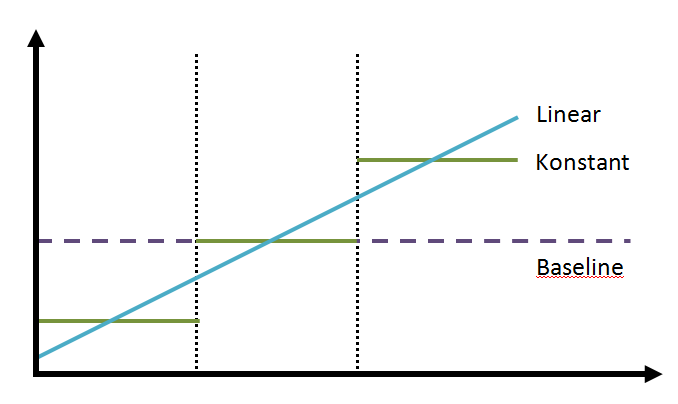
\includegraphics[width=0.8\textwidth]{SessionTypen.png}
  \caption[Vergleich der Geschwindigkeitsfunktionen]{Zeigt Relation zwischen
  Baseline konstanter und linearer Funktion. Die konstante Funktion hat innerhalb einer Runde (gestrichelte Linie) stets die gleiche
mittlere Geschwindigkeit wie die lineare Funktion.\\
  TODO Vektorgrafik}
  \label{fig:SessionTypen}
\end{center}
\end{figure} 

\subsection{Menüsystem im Spiel}
Zur schnellen Entwicklung der Benutzerschnittstellen wurde auf den
vollständigen Eigenbau eines Menüsystems verzichtet und stattdessen eine dünne Kompatibilitätsschicht
eingeführt, die es ermöglicht, die bestehende Swing-Bibliothek von Java für die
Benutzerschnittstelle des Spiels über die 3D-Umgebung zu legen. Dadurch kann die
Benutzerschnittstelle wie gewohnt entwickelt und separat getestet werden, ohne auf die
besonderen Herausforderungen Rücksicht nehmen zu müssen, die es mit sich bringt, wenn
man grafische Elemente wie Buttons, Radio-/Checkboxen und Scrollleisten in einer 3D-
Umgebung verwenden möchte.

Die hierfür entwickelte Kompatibilitätsschicht (\texttt{OffscreenJPanel})
zeichnet alle Swing- Komponenten in ein transparentes Bild, dass dann über die 3D-Umgebung des Spiels
gelegt wird. Alle Maus- und Tastatureingaben auf diesem Bild werden abgefangen und an
die eigentlichen Swing-Komponenten weitergeleitet. Während der Spieler das Raumschiff
steuert, wird das komplette Swing-System ausgeblendet, was die Performance des Spiels
verbessert.

Um den zugrundeliegenden Ablauf des Spiels intuitiv programmieren zu können, wurde
aufbauend auf die o.g. Kompatibilitätsschicht ein Menüsystem (GameMenu, MenuScreen
und das Package \texttt{ui.screen}) entwickelt, dass die von Spielen typische
Abfolge von "`Bildschirmen"' erleichtert, zwischen denen der Spieler sich auf vordefinierten Pfaden
bewegen kann.

\subsection{Persistenz von Benutzereinstellungen}
Das Spiel bietet die Möglichkeit, die Sounds an- und abzustellen sowie die Steuerung zu
invertieren, so dass die Auf/Ab-Pfeile sich wahlweise wie bei einem Flugzeugsimulator oder
Rennspiel verhalten. Um diese Einstellungen persistent zu halten, verwendet das Applet die
LiveConnect-Funktionalität moderner Webbrowser, mit denen es Javascript-Code im das
Applet umgebenden HTML-Dokument aufrufen kann. Dort werden die Einstellungen dann
als Cookie abgelegt und beim wiederholten Starten des Spiels automatisch ausgelesen.

\subsection{RPC-Eigenbau Serialisierung über HTTP mit Java
Objekt-Serialisierung}
Für die Kommunikation des Spielapplets mit dem
Spielserver wurde ein RPC\footnote{Remote Procedure Call, das Aufrufen von
Programmcode auf einem anderen Computersystem.}-Mecha\-nismus entwickelt, der
sowohl einfach zu verwenden ist als auch problemlos über das Internet funktioniert. Als Grundlage dient die HTTP-Verbindung zum Spielserver, über die bereits
das Spiel selbst bestehend aus Programmcode, Grafiken, Sounds, usw. geladen wird.
Will das Spiel nun im Ablauf weitere Daten vom Spielserver empfangen oder an diesen
senden, werden diese als Java-Objekte übergeben und serialisiert. Dies ergibt einen binären
Blob, der als Dateiupload an den Server übertragen wird, der diesen Blob dort wieder
deserialisiert um das ursprüngliche Java-Objekt zu erhalten. Abhängig von der auf dem
Spielserver aufgerufenen URL, wird dieses Java-Objekt auf dem Server einem bestimmten
Teil der Programmlogik übergeben, die dann damit arbeitet. Eventuelle
Rückgabewerte der Programmlogik werden nach dem gleichen Verfahren durch Serialisierung von Objekten
in binäre Blobs umgewandelt, als Dateidownload dem Spielapplet übermittelt und dort
wieder in ein Java-Objekt deserialisiert. Aus Sicherheitsgründen werden auf dem Server
auftretende Fehler nicht an das Spiel übergeben und nur in ein Logfile auf dem Server
geschrieben; so wird das versehentliche Anzeigen bspw. von Passwörtern oder der
Datenbankstruktur auf der Clientseite vermieden.

\subsection{Java3D}
Flowgame ist eine Java3D\footnote{Einführung unter
\url{http://java.sun.com/developer/onlineTraining/java3d/}}-Anwendung, die als
Java-Applet im Browser des Spielers (also auf dem Client) läuft. Das Universum bei Flowgame enthält vier unterschiedliche Typen von dreidimensionalen Objekten. Einen Tunnel, durch den das Raumschiff des Spielers fliegt,
wobei es den entgegenkommenden Asteroiden ausweichen und Diamanten aufsammeln
soll.

Die folgende Beschreibung bezieht sich auf den Stand von Revision 866.
Alle Klassen der 3D-Engine befinden sich im Package \texttt{client.engine}.

Während dem Start des Applets wird in \texttt{GameApplet.java} (Zeile 79) der
Szenengraph für das Spiel erstellt. Dort wird ein \texttt{Game3D} Objekt
erzeugt, dass die einzelnen 3D-Objekte erstellt und in einen Szenengraph
einhängt. In \texttt{Game3D.java} wird in Zeile 151 zunächst das Universum
selbst instanziiert. Der Methodenaufruf in Zeile 162 erstellt die restlichen Objekte und bindet sie ein. Der Tunnel wird dabei (in Tunnel.java) mittels
Javacode als zylinderförmige \texttt{Shape3D} erzeugt, während die anderen
Objekte aus externen Objektmodelldateien eingelesen werden. Diese Objektmodelldateien befinden sich im
Ressourcen Ordner (\texttt{src/res}).

Schiffsbewegung, Steuerung und Kollisionserkennung wird mit Behaviors realisiert.
Behaviors dienen bei Java3D als Basis für Interaktion und Animation. Viele dieser Aktionen
müssen in jedem Frame ausgeführt oder aufgerufen werden. Daher gibt es eine abstrakte
\texttt{RepeatingBehavior} Klasse, die beim Neuzeichnen jedes Frames aufgerufen
wird und den Zeitabstand zwischen den Frames misst. Letzteres ermöglicht eine Steuerung der
Geschwindigkeit unabhängig von der Framerate. Gleichzeitig implementiert diese abstrakte
Klasse das Interface \texttt{GameListener}, mit dem auf Ereignisse im
Spielablauf reagiert werden kann.

\texttt{ShipNavigationBehavior} dient zur Bewegung des Schiffes in xy-Richtung,
also nach links/ rechts und oben/unten. Die z-Achse entspricht bei Java3D der Tiefeninformation, Bewegung
in dieser Richtung wird mit der \texttt{ForwardBehavior} realisiert, wobei die
Geschwindigkeit der Bewegung wiederum von der \texttt{SpeedChangeBehavior}
gesteuert wird. Über diese Behavior wird der Schwierigkeitsgrad reguliert. Die
Kamera folgt dem Schiff dabei in festem Abstand, es sieht also so aus, als ob die Kollisionsobjekte (Diamanten, Asteroiden) auf den Spieler zukommen. Die
\texttt{CreateCollidablesBehavior} stellt sicher, dass vor dem Schiff immer wieder neue Kollisionsobjekte erzeugt werden.

Da die bei Java3D eingebauten Möglichkeiten zur Kollisionserkennung vor allem bei
höheren Bewegungsgeschwindigkeiten des Schiffes versagen, wurde auch eine eigene
(einfache) Kollisionserkennung in Form der \texttt{CollisionBehavior}
implementiert. Der (unendlich lange) Tunnel bewegt sich selbst nicht, die Illusion der Bewegung wird über eine
Texturtransformation gesteuert. Die \texttt{TextureTransformBehavior} sorgt
dafür, dass die Geschwindigkeit der Textur, zu der des Schiffes passt.

Die Behaviors werden bei der Erzeugung des 3D-Universums (s.o.) an die jeweilig
betroffenen Objekte gebunden.

\section{Entwicklungsumgebung}
Die Entwicklungsumgebung beinhaltet alle Programme, die zum entwerfen,
programmieren, kompilieren und testweisen ausführen des Spiels und der Verwaltung des
Entwicklungsprozesses nötig sind.

Für eine zentrale Verwaltung des gesamten Codes und aller weiteren Bestandteile des
Spiels (Grafiken, Musik, Sounds) wurde auf Google Code ein Projekt angelegt, dass neben
dem Versionskontrollsystem Subversion auch ein Issue-Tracking für das Verfolgen und
Verwalten von Fehlern und Änderungswünschen bietet.

Als IDE\footnote{Integrated Development Environment -- integrierte
Entwicklungsumgebung} wird Eclipse in der EE\footnote{Enterprise
Edition, ermöglicht unter anderem das Entwickeln von Webanwendungen}-Variante
mit diversen Erweiterungen verwendet: Subclipse stellt die Anbindung an das von Google Code zur Verfügung gestellten Versionkontrollsystem bereit, FindBugs und PMD analysieren den Programmcode auf häufig auftretende Programmierfehler.
Um das Spiel vollständig lokal auszuführen, wird ein lokal installierter MySQL-
Datenbankserver notwendig. So können Änderungen ohne Beeinflussung des auf Facebook
laufenden Spiels getestet werden.

Um jederzeit eine lauffähige Version des neuesten Entwicklungsstands zu haben, wird
Hudson als CI\footnote{Continuous Integration, das durchgängige Kompilieren und Auswerten von Programmcode}-Server verwendet, der zum einen die o.g. Werkzeuge FindBugs
und PMD nochmals zentral ausführt und dazu Statistiken erzeugt und zum anderen das
Deployment des Spiels auf den Facebook bekannten Spielserver vollständig automatisiert
und reproduzierbar durchführen kann. Insgesamt verbessert der CI-Server damit die Code-
Qualität und reduziert etwaige Fehlhandlungen beim Deployment neuer Versionen des
Spiels, wodurch weniger Fehler im Spiel selbst auftreten.

\section{Herausforderungen bei der Umsetzung}

\begin{itemize}
  \item Plattformübergreifende Laufzeit
  	\begin{itemize}
    	\item[$\circ$] Java Runtime + Plugin (insb. MacOSX)
    	\item[$\circ$] Java3D
		\item[$\circ$] Tastatur-Events auf versch. OS
		\item[$\circ$] Facebook API-Änderungen (Einladungen, App-Einbindung)
  	\end{itemize}
\item Projektmanagement
	\begin{itemize}
  		\item[$\circ$] zu spät mit Issue Tracking angefangen
  		\item[$\circ$] Zeitbudget/Auslastung Teammitglieder während Studium
  		\item[$\circ$] unscharfe Anforderungen wurden zu spät festgezurrt
	\end{itemize}
\end{itemize}

%\usepackage{graphics} is needed for \includegraphics
\begin{figure}[htp]
\begin{center}
  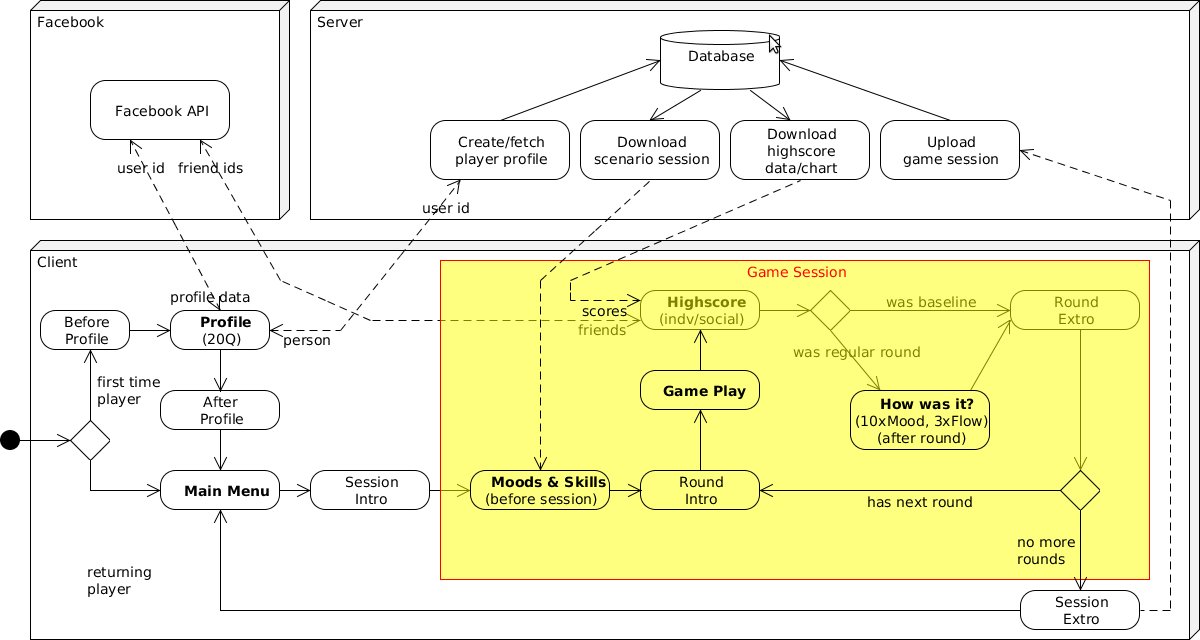
\includegraphics[width=\textwidth]{Gesamtablauf.png}
  \caption[Gesamtablauf]{Gesamtablauf\\
TODO: Phil: Muss noch auf deutsch, Mauszeiger raus und an finalen Ablauf anpassen}
  \label{fig:Gesamtablauf}
\end{center}
\end{figure} 

\markboth{Abk�rzungsverzeichnis}{Abkürzungsverzeichnis}
\section*{Abk�rzungsverzeichnis}
\addcontentsline{toc}{section}{Abkürzungsverzeichnis}
\begin{acronym}
\acro{DV}{Document Verifier}
\acrodefplural{DV}[DV]{Document Verifiern}
\end{acronym}

\clearpage

\clearpage
\addcontentsline{toc}{section}{Abbildungen}
\listoffigures
  
\clearpage
\addcontentsline{toc}{section}{Literatur}
\bibliography{literatur}{}
\bibliographystyle{alphadin}

\end{document}
